\section{Piecewise Affine Warping}

In the previous sections we established the mathematical and geometric prerequisites for feature-based face morphing: we can detect and align facial landmarks, we understand how to decompose a face into a Delaunay triangulation, and we know how to compute affine transformations and barycentric coordinates. In this section we combine all of these ingredients into the core rendering engine of the morphing pipeline: \textbf{piecewise affine warping}.

\subsection{The Concept}

The central idea is conceptually simple but computationally powerful. Once we have:
\begin{enumerate}
    \item A set of corresponding landmarks on Face~A and Face~B,
    \item A Delaunay triangulation computed on a \emph{mean shape} (defined below),
    \item The theory to compute an affine transform between any two corresponding triangles,
\end{enumerate}
we can \emph{warp} each input face into a common geometric frame.

For every triangle in the mean-shape mesh, we compute two independent affine transforms: one that maps the corresponding triangle in Face~A to the mean triangle, and another that maps the corresponding triangle in Face~B to the mean triangle. Applying these transforms pixel-by-pixel renders both faces so that their facial features (eyes, nose, mouth, jawline) are perfectly aligned to the intermediate geometry. Because affine transformations are linear, they preserve straight lines along triangle edges, which guarantees that adjacent triangles meet seamlessly without visible seams or discontinuities. This is why the method is called \emph{piecewise} affine: globally non-rigid, but locally affine within each triangle.

\begin{figure}[h]
\centering
\begin{tikzpicture}[>=stealth, line width=0.8pt, scale=1.1]
    % Source Triangle
    \coordinate (A1) at (0,0);
    \coordinate (A2) at (3.2,0.4);
    \coordinate (A3) at (1.8,2.6);
    \draw[thick, blue, fill=blue!8] (A1) -- (A2) -- (A3) -- cycle;
    \fill[blue] (A1) circle (2pt) node[below left] {$\mathbf{a}_i$};
    \fill[blue] (A2) circle (2pt) node[below right] {$\mathbf{a}_j$};
    \fill[blue] (A3) circle (2pt) node[above] {$\mathbf{a}_k$};
    \node[blue, font=\small] at (1.6, -0.6) {Face~A (Source)};

    % Arrow
    \draw[->, thick, orange] (3.7, 1.3) -- node[above, pos=0.5, sloped] {\small $\mathbf{H}_A$} (5.3, 1.3);

    % Mean Triangle
    \coordinate (M1) at (6, 0.2);
    \coordinate (M2) at (8.4, 0.8);
    \coordinate (M3) at (7.2, 2.4);
    \draw[thick, green!60!black, fill=green!8] (M1) -- (M2) -- (M3) -- cycle;
    \fill[green!60!black] (M1) circle (2pt) node[below left] {$\mathbf{m}_i$};
    \fill[green!60!black] (M2) circle (2pt) node[below right] {$\mathbf{m}_j$};
    \fill[green!60!black] (M3) circle (2pt) node[above] {$\mathbf{m}_k$};
    \node[green!60!black, font=\small] at (7.2, -0.5) {Mean Shape (Target)};

    % Matrix box
    \node[draw, rounded corners, fill=orange!10, inner sep=4pt, font=\small] at (4.5, 2.6) {
        $\mathbf{H}_A = \begin{bmatrix}
            h_{11} & h_{12} & t_x \\
            h_{21} & h_{22} & t_y \\
            0 & 0 & 1
        \end{bmatrix}$
    };
    \draw[->, orange, dashed] (4.5, 2.3) -- (4.5, 1.8);
\end{tikzpicture}
\caption{Single-triangle affine warp. Three landmark correspondences determine a unique $3 \times 3$ homogeneous matrix $\mathbf{H}_A$ that maps the source triangle in Face~A to the corresponding triangle in the mean shape. The top two rows of $\mathbf{H}_A$ form the standard $2 \times 3$ affine warp matrix used in image processing.}
\label{fig:single-triangle-warp}
\end{figure}

\subsection{Computing the Mean Shape}

The first step is to define the common target geometry. Given two sets of corresponding landmarks
\[
    L_A = \{\mathbf{a}_1, \mathbf{a}_2, \ldots, \mathbf{a}_n\}, \quad
    L_B = \{\mathbf{b}_1, \mathbf{b}_2, \ldots, \mathbf{b}_n\},
\]
where each $\mathbf{a}_i, \mathbf{b}_i \in \mathbb{R}^2$ are 2D image coordinates, the \emph{mean shape} is simply the arithmetic average of corresponding points:
\begin{equation}
    \mathbf{m}_i = \frac{\mathbf{a}_i + \mathbf{b}_i}{2}, \quad i = 1, \ldots, n.
\end{equation}
The complete mean landmark set is $M = \{\mathbf{m}_1, \ldots, \mathbf{m}_n\}$. This symmetric average places the target geometry exactly halfway between the two faces, which is ideal for a 50/50 morph.

More generally, one can define a \emph{weighted} mean shape:
\begin{equation}
    \mathbf{m}_i(\alpha) = (1 - \alpha)\,\mathbf{a}_i + \alpha\,\mathbf{b}_i, \quad \alpha \in [0, 1],
\end{equation}
where $\alpha = 0$ yields the original Face~A geometry, $\alpha = 1$ yields Face~B, and $\alpha = 0.5$ recovers the simple average. In a full morphing pipeline, $\alpha$ is varied smoothly from 0 to 1 to produce the intermediate frames of the animation.

\subsection{The Triangular Correspondence}

Once the mean landmarks $M$ are computed, we run Delaunay triangulation on them. The triangulation yields a set of triangles
\[
    \mathcal{T}_{\text{mean}} = \{ T_{\text{mean}}^{(1)}, T_{\text{mean}}^{(2)}, \ldots, T_{\text{mean}}^{(K)} \},
\]
where each triangle is defined by three vertex indices: $T_{\text{mean}}^{(p)} = (\mathbf{m}_i, \mathbf{m}_j, \mathbf{m}_k)$.

Because the triangulation is computed on the \emph{indices} of the landmarks, the same index triplet automatically defines corresponding triangles in the source faces:
\begin{align*}
    T_A^{(p)} &= (\mathbf{a}_i, \mathbf{a}_j, \mathbf{a}_k), \\
    T_B^{(p)} &= (\mathbf{b}_i, \mathbf{b}_j, \mathbf{b}_k).
\end{align*}
This index-preserving mapping guarantees \emph{topological consistency}: every triangle in the mean mesh has exactly one counterpart in Face~A and one in Face~B, with matching vertex orderings. This one-to-one correspondence is what makes the affine warp well-defined and computationally straightforward.

\begin{figure}[h]
\centering
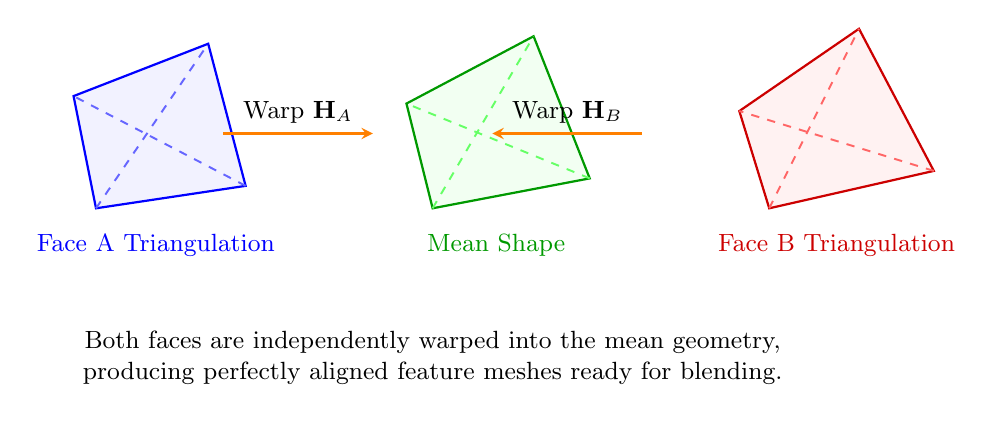
\begin{tikzpicture}[>=stealth, line width=0.7pt, scale=0.95]
    % Face A (Left)
    \begin{scope}[shift={(-4.5, 0)}]
        \coordinate (A1) at (0,0);
        \coordinate (A2) at (2,0.3);
        \coordinate (A3) at (1.5,2.2);
        \coordinate (A4) at (-0.3,1.5);
        \draw[thick, blue, fill=blue!5] (A1) -- (A2) -- (A3) -- (A4) -- cycle;
        \draw[dashed, blue!60] (A1) -- (A3);
        \draw[dashed, blue!60] (A2) -- (A4);
        \node[blue, font=\small] at (0.8, -0.5) {Face~A Triangulation};
    \end{scope}

    % Face B (Right)
    \begin{scope}[shift={(4.5, 0)}]
        \coordinate (B1) at (0,0);
        \coordinate (B2) at (2.2,0.5);
        \coordinate (B3) at (1.2,2.4);
        \coordinate (B4) at (-0.4,1.3);
        \draw[thick, red!80!black, fill=red!5] (B1) -- (B2) -- (B3) -- (B4) -- cycle;
        \draw[dashed, red!60] (B1) -- (B3);
        \draw[dashed, red!60] (B2) -- (B4);
        \node[red!80!black, font=\small] at (0.9, -0.5) {Face~B Triangulation};
    \end{scope}

    % Mean Shape (Center)
    \begin{scope}[shift={(0, 0)}]
        \coordinate (M1) at (0,0);
        \coordinate (M2) at (2.1,0.4);
        \coordinate (M3) at (1.35,2.3);
        \coordinate (M4) at (-0.35,1.4);
        \draw[thick, green!60!black, fill=green!5] (M1) -- (M2) -- (M3) -- (M4) -- cycle;
        \draw[dashed, green!60] (M1) -- (M3);
        \draw[dashed, green!60] (M2) -- (M4);
        \node[green!60!black, font=\small] at (0.85, -0.5) {Mean Shape};
    \end{scope}

    % Arrows
    \draw[->, thick, orange] (-2.8, 1.0) -- node[above, sloped, black, font=\small] {Warp $\mathbf{H}_A$} (-0.8, 1.0);
    \draw[<-, thick, orange] (0.8, 1.0) -- node[above, sloped, black, font=\small] {Warp $\mathbf{H}_B$} (2.8, 1.0);

    % Bottom caption
    \node[align=center, font=\small] at (0, -2.0) {Both faces are independently warped into the mean geometry,\\ producing perfectly aligned feature meshes ready for blending.};
\end{tikzpicture}
\caption{Complete warping concept. The Delaunay triangulation is computed once on the mean shape. The same connectivity is projected onto both input faces via index correspondence. Each face is then warped into the mean geometry using its own set of piecewise affine transforms, aligning all facial features without distortion discontinuities.}
\label{fig:complete-warp-concept}
\end{figure}

\subsection{Computing the Affine Warp for Each Triangle}

For a given triangle $T_A^{(p)} = (\mathbf{a}_i, \mathbf{a}_j, \mathbf{a}_k)$ and its target $T_{\text{mean}}^{(p)} = (\mathbf{m}_i, \mathbf{m}_j, \mathbf{m}_k)$, we seek an affine transform that maps every point inside the source triangle to the target triangle. In homogeneous coordinates, a 2D affine transform is represented by a $3 \times 3$ matrix:
\begin{equation}
    \begin{bmatrix} x' \\ y' \\ 1 \end{bmatrix}
    =
    \mathbf{H}
    \begin{bmatrix} x \\ y \\ 1 \end{bmatrix},
    \quad \text{where} \quad
    \mathbf{H} =
    \begin{bmatrix}
        h_{11} & h_{12} & t_x \\
        h_{21} & h_{22} & t_y \\
        0 & 0 & 1
    \end{bmatrix}.
\end{equation}
The top-left $2 \times 2$ block handles rotation, scaling, and shearing; the rightmost column handles translation.

Because three non-collinear points uniquely determine a 2D affine transform, we can solve for $\mathbf{H}_A$ by stacking the three vertex correspondences into a matrix equation:
\begin{equation}
    \underbrace{
    \begin{bmatrix}
        m_{ix} & m_{jx} & m_{kx} \\
        m_{iy} & m_{jy} & m_{ky} \\
        1 & 1 & 1
    \end{bmatrix}}_{\mathbf{X}_{\text{mean}}}
    =
    \mathbf{H}_A
    \underbrace{
    \begin{bmatrix}
        a_{ix} & a_{jx} & a_{kx} \\
        a_{iy} & a_{jy} & a_{ky} \\
        1 & 1 & 1
    \end{bmatrix}}_{\mathbf{X}_A}.
\end{equation}
Assuming the source triangle is non-degenerate (its vertices are not collinear), $\mathbf{X}_A$ is invertible. We solve for the forward warp matrix:
\begin{equation}
    \mathbf{H}_A = \mathbf{X}_{\text{mean}} \, \mathbf{X}_A^{-1}.
\end{equation}
The exact same procedure yields $\mathbf{H}_B = \mathbf{X}_{\text{mean}} \, \mathbf{X}_B^{-1}$ for Face~B. The explicit inverse of a $3 \times 3$ matrix can be computed via cofactors, Cramer's rule, or standard numerical routines. For the affine case, the bottom row of $\mathbf{H}_A$ is always $(0, 0, 1)$, so in practice we only need to invert the $2 \times 3$ augmented system or solve two independent $3 \times 3$ linear systems for the $x$ and $y$ components separately.

\subsection{Inverse Warping (Backward Mapping)}

A naive approach would apply the forward transform $\mathbf{H}_A$ to every pixel inside $T_A^{(p)}$ and write the color to the corresponding location in the output image. This \emph{forward mapping} has a critical flaw: the transformed coordinates will almost always fall between integer pixel locations, and multiple source pixels may map to the same destination or leave destination pixels completely unassigned. The result is a warped image with \emph{holes} and overlapping samples.

The standard solution is \emph{inverse warping} (also called backward mapping). Instead of asking ``where does this source pixel go?'', we ask ``which source pixel belongs to this destination pixel?''. The procedure is:

\begin{enumerate}
    \item Allocate a blank output image $W$ with the same dimensions as the mean shape canvas.
    \item Precompute the \emph{inverse} affine matrices $\mathbf{H}_A^{-1}$ and $\mathbf{H}_B^{-1}$ for every triangle. These map from the mean shape \emph{back} to the original face geometry.
    \item For each output pixel at integer coordinates $(x, y)$:
    \begin{enumerate}
        \item \textbf{Locate} which mean triangle $T_{\text{mean}}^{(p)}$ contains $(x, y)$.
        \item \textbf{Back-project} using the inverse matrix:
        \begin{equation}
            \begin{bmatrix} x_s \\ y_s \\ 1 \end{bmatrix}
            = \mathbf{H}_A^{-1}
            \begin{bmatrix} x \\ y \\ 1 \end{bmatrix}.
        \end{equation}
        This yields continuous (non-integer) source coordinates $(x_s, y_s)$.
        \item \textbf{Sample} the source image $I_A$ at $(x_s, y_s)$ using bilinear interpolation.
        \item \textbf{Write} the interpolated color value to $W(x, y)$.
    \end{enumerate}
\end{enumerate}

Because we visit every output pixel exactly once and fill it via back-projection, inverse warping \emph{guarantees} a complete, hole-free image.

\paragraph{Bilinear Interpolation.}
Since $(x_s, y_s)$ are real-valued coordinates, we sample the four nearest integer pixels and blend them according to their fractional distances. Let $x_0 = \lfloor x_s \rfloor$, $y_0 = \lfloor y_s \rfloor$, $u = x_s - x_0$, and $v = y_s - y_0$. The interpolated intensity is:
\begin{align}
    I(x_s, y_s) =\; &(1-u)(1-v)\, I(x_0, y_0) \;+\; u(1-v)\, I(x_0+1, y_0) \nonumber \\
                  &+\; (1-u)v\, I(x_0, y_0+1) \;+\; uv\, I(x_0+1, y_0+1).
\end{align}
This formula is applied independently to each color channel (R, G, B). Bilinear interpolation produces smooth gradients and avoids the blocky artifacts of nearest-neighbor sampling, while remaining computationally cheap.

\subsection{Point-in-Triangle Test Using Barycentric Coordinates}

Step 3(a) above requires an efficient way to determine which triangle ``owns'' a given output pixel. Barycentric coordinates, introduced in Section~3, serve this purpose elegantly.

For a target point $\mathbf{p} = (x, y)$ and a mean triangle with vertices $\mathbf{m}_i, \mathbf{m}_j, \mathbf{m}_k$, we compute the barycentric weights $(w_i, w_j, w_k)$ by solving:
\begin{equation}
    \mathbf{p} = w_i \mathbf{m}_i + w_j \mathbf{m}_j + w_k \mathbf{m}_k,
    \quad \text{subject to} \quad w_i + w_j + w_k = 1.
\end{equation}
This is a $2 \times 2$ linear system (after eliminating $w_k = 1 - w_i - w_j$) that can be solved analytically using cross-products or determinants. The membership test is then trivial:
\begin{equation}
    \mathbf{p} \in T_{\text{mean}}^{(p)} \quad \Longleftrightarrow \quad
    0 \leq w_i \leq 1 \;\land\; 0 \leq w_j \leq 1 \;\land\; 0 \leq w_k \leq 1.
\end{equation}
Since the weights sum to one, it is sufficient to check that all three are non-negative. If the condition holds, the point lies inside (or exactly on the edge of) the triangle. Additionally, these same weights can be reused for texture coordinate interpolation if needed, though for pure color warping we rely on the inverse matrix.

\subsection{Bounding Box Optimization}

Testing every output pixel against every triangle would result in $\mathcal{O}(N_{\text{pixels}} \times N_{\text{triangles}})$ complexity, which is prohibitively slow for high-resolution images. We can dramatically accelerate this using a \emph{bounding box} culling strategy:

\begin{enumerate}
    \item For each mean triangle $T_{\text{mean}}^{(p)}$, compute its axis-aligned bounding box (AABB):
    \[
        x_{\min} = \lfloor \min(m_{ix}, m_{jx}, m_{kx}) \rfloor, \quad
        x_{\max} = \lceil \max(m_{ix}, m_{jx}, m_{kx}) \rceil,
    \]
    and similarly for $y_{\min}, y_{\max}$.
    \item Iterate \emph{only} over integer pixels $(x, y)$ satisfying $x_{\min} \leq x \leq x_{\max}$ and $y_{\min} \leq y \leq y_{\max}$.
    \item Perform the barycentric point-in-triangle test only for pixels inside the bounding box.
\end{enumerate}

Since a triangle's bounding box typically contains only a small constant factor more pixels than the triangle itself, this reduces the effective complexity to nearly $\mathcal{O}(N_{\text{pixels}})$ overall: each output pixel is tested against only the few triangles whose bounding boxes overlap it, and exactly one test succeeds. This optimization is standard in all GPU and software rasterizers.

\subsection{Handling the Background}

The Delaunay triangulation covers exactly the \emph{convex hull} of the landmark set. Everything outside this hull---hair, ears, neck, shoulders, and background---falls outside all triangles and will remain unfilled after the warping step. Several strategies exist to handle these regions:

\begin{description}
    \item[Direct Passthrough (Copy Original):] For pixels outside the convex hull, simply copy the original unwarped pixel from Face~A (or Face~B). This is the simplest approach and works well when the background is uniform or when the hull tightly covers the face. The transition at the hull boundary may show a slight geometric discontinuity if the face edge aligns poorly with the outermost landmarks.

    \item[Extended Triangulation with Border Points:] Add four artificial ``corner'' landmarks at the image boundaries (e.g., $(0,0), (W,0), (W,H), (0,H)$) and optionally midway points along each edge. Recompute the Delaunay triangulation including these points. The triangles connecting the convex hull to the image border form a smooth extension field that gently warps the background towards the mean shape, eliminating hard cutoff lines.

    \item[Masking and Alpha Compositing:] Render the warped face into a separate layer with an alpha mask derived from the convex hull. Composite this layer over an unwarped background layer using standard alpha blending:
    \[
        C_{\text{final}} = \alpha \, C_{\text{warped}} + (1 - \alpha) \, C_{\text{background}},
    \]
    where $\alpha = 1$ inside the hull and smoothly feathers to $0$ near the boundary. This gives the most control over edge appearance and is the standard approach in professional morphing software.
\end{description}

In practice, a hybrid approach works best: extend the triangulation with border points to cover the entire image, then apply the piecewise warp uniformly. Triangles far from the face landmarks undergo nearly identity transforms, preserving the background naturally while ensuring complete pixel coverage.

\subsection{Complete Warping Procedure}

Algorithm~\ref{alg:piecewise-warp} summarizes the full piecewise affine warping pipeline for a single input face. Running it twice (once for Face~A, once for Face~B) produces two geometrically aligned images ready for cross-dissolve blending.

\begin{figure}[h]
\centering
\fbox{\begin{minipage}{0.9\textwidth}
\textbf{Algorithm:} Piecewise Affine Inverse Warp\\[4pt]
\textbf{Input:} Source image $I$, landmarks $L_{\text{src}} = \{\mathbf{a}_1, \dots, \mathbf{a}_n\}$, mean landmarks $M = \{\mathbf{m}_1, \dots, \mathbf{m}_n\}$, triangulation $\mathcal{T}$\\
\textbf{Output:} Warped image $W$ in mean shape geometry
\begin{enumerate}
    \item Initialize $W$ as a blank image with the canvas dimensions.
    \item \textbf{For each} triangle index $p = 1$ to $K$ in $\mathcal{T}$:
    \begin{enumerate}
        \item Retrieve vertex indices $(i, j, k)$ for triangle $p$.
        \item Construct $\mathbf{X}_{\text{src}}$ from $\mathbf{a}_i, \mathbf{a}_j, \mathbf{a}_k$ and $\mathbf{X}_{\text{mean}}$ from $\mathbf{m}_i, \mathbf{m}_j, \mathbf{m}_k$.
        \item Compute forward matrix: $\mathbf{H}^{(p)} = \mathbf{X}_{\text{mean}} \, \mathbf{X}_{\text{src}}^{-1}$.
        \item Compute inverse matrix: $\mathbf{H}_{\text{inv}}^{(p)} = \left(\mathbf{H}^{(p)}\right)^{-1}$.
        \item Compute bounding box $(x_{\min}, x_{\max}, y_{\min}, y_{\max})$ of $T_{\text{mean}}^{(p)}$.
    \end{enumerate}
    \item \textbf{For each} triangle $p = 1$ to $K$:
    \begin{enumerate}
        \item \textbf{For} $y$ from $y_{\min}$ to $y_{\max}$:
        \item \quad \textbf{For} $x$ from $x_{\min}$ to $x_{\max}$:
        \begin{enumerate}
            \item Compute barycentric weights $(w_i, w_j, w_k)$ of $(x, y)$ relative to $T_{\text{mean}}^{(p)}$.
            \item \textbf{If} $w_i \geq 0$ and $w_j \geq 0$ and $w_k \geq 0$:
            \begin{enumerate}
                \item Back-project: $\begin{bmatrix} x_s \\ y_s \\ 1 \end{bmatrix} = \mathbf{H}_{\text{inv}}^{(p)} \begin{bmatrix} x \\ y \\ 1 \end{bmatrix}$.
                \item Sample source: $C = \text{BilinearInterp}(I, x_s, y_s)$.
                \item Write output: $W(x, y) \gets C$.
            \end{enumerate}
        \end{enumerate}
    \end{enumerate}
    \item \textbf{Return} $W$.
\end{enumerate}
\end{minipage}}
\caption{Complete piecewise affine inverse warping algorithm. The affine matrices and bounding boxes are precomputed once per triangle (Step 2), then the rasterization loop (Step 3) fills the output image efficiently.}
\label{alg:piecewise-warp}
\end{figure}

The computational cost is dominated by Step 3, which touches every pixel in the convex hull exactly once. With $K$ triangles and image resolution $H \times W$, the complexity is $\mathcal{O}(HW + K)$, where the linear term comes from matrix precomputation and the dominant $HW$ term comes from pixel-level sampling. In typical face morphing, $K \approx 100\text{--}200$ triangles and $HW \approx 10^6$ pixels, making the per-frame warp easily real-time on modern hardware.